\documentclass[conference]{IEEEtran}
\usepackage{cite}
\usepackage{amsmath,amssymb,amsfonts}
\usepackage{algorithmic}
\usepackage{graphicx}
\usepackage{textcomp}
\usepackage{xcolor}
\usepackage{colortbl}
\usepackage{multirow}
\usepackage[export]{adjustbox}
\def\BibTeX{{\rm B\kern-.05em{\sc i\kern-.025em b}\kern-.08em
    T\kern-.1667em\lower.7ex\hbox{E}\kern-.125emX}}
\begin{document}

\title{
    Vad är en bra projektmetod för små IT-projekt?\\
{\normalsize Ett försök att besvara frågan görs i kursen II1302 "Projekt och projektmetoder"
vid KTH EECS Kista våren 2019}

% To accommodate for the .doc's formatting, the author blocks have been replaced with this section instead.
\begin{center}
    \large{ 
        First Author\textsuperscript{1}, Second Author\textsuperscript{2}, 
        Third Author\textsuperscript{3}\\
        \textit{\\First-Third Department, First-Third University\\
                Address Including Country Name\\}
        \textsuperscript{1}\texttt{first.author@first-third.edu}\\
        \textsuperscript{3}\texttt{first.author@first-third.edu}\\
        \textit{Second Company\\
        Address Including Country Name\\}
        \textsuperscript{2}\texttt{second.author@second.com}
    }
\end{center}
}

% This is just to kill the warning about no author given.
\author{}

\maketitle

\begin{abstract}
Syfte och mål med kursen - "Vad är en bra projektmetod för små IT-projekt?" Kursens metod för att uppnå
kursens syfte och mål. Resultat av kursens metod - uppfylls syfte och mål med kursen.\\
Kan undersökningsfrågan besvaras?
\end{abstract}

\begin{IEEEkeywords}
IoT, JavaScript, Personsökare, Pager, Connected devices
\end{IEEEkeywords}

\section{Om detta dokument och undersökning}
Vem är läsaren? Dokumentets disposition (istället för innehållsförteckning). Vilken trovärdighet har innehållet?

Projektets resultat (framtagen produkt) framgår av bilagorna.

Bilagor.


\section{Introduktion}
Om detta kapitel \dots

\subsection{Bakgrund}
Mer om kursen, syfte och mål. Allmänt om IT-projekt. Undersökningsfrågan.

\subsection{Problemformulering}
Övergripande frågeställning.
Vad menas med en bra projektmetod? Åstadkommer/skapar projeket rätt saker och konstrueras
lösningar på bästa sätt?

\subsection{Undersökningsstrategi/lösningsstrategi}
Fallstudie genom att i grupp försöka genomföra ett mindre IT-projekt med utvalda projektmetoder
och där varje gruppmedlem värderar sitt ansvarsområde i projektet för att ur detta försöka
besvara den övergripande frågeställningen.

\subsection{Relaterade arbeten}
Lorem ipsum.

\subsection{Avgränsningar}
Dolor sit.

\section{Teori och ingenjörspraxis.}
Detta kapitel listar och i viss mån beskriver teorier och ingenjörspraxis som använts
i undersökningen. Det finns två underkapitel, litteraturstudie och förstudie.

\subsection{Litteraturstudie.}
I detta kapitel anges litteratur och andra källor som har använts för att hitta ingångar
och möjligheter i undersökningen. Förutom de källor som anges finns förmodligen andra 
och kanske bättre källor som denna studie inte använt sig av.

Undersökningen görs utifrån övergripande projektmetoder men också utifrån specifika metoder
och arbetssätt som används av olika kompetenser i projektets team. Vilka dessa kompetenser
är framgår av texten nedan.

\textbf{Övergripande källor}
\begin{itemize}
    \item Projektets hälsa och status
    \item Scrum
    \item Fasindelning
    \item Projektgrunder
    \item Person och gruppdynamik
\end{itemize}

\textbf{Kundrepresentant} - kompetens enligt [Essence 1.0]
\begin{itemize}
    \item Vision
    \item Kravspecifikation
    \begin{itemize}
        \item "Stories
        \item "UseCase"
    \end{itemize}
\end{itemize}

\textbf{Analytiker} - kompetens enligt ...
\begin{itemize}
    \item Arkitektur (Kruchten, 1995)
\end{itemize}

\textbf{Utvecklare} - kompetens enligt ...
\begin{itemize}
    \item Designplan
\end{itemize}

\textbf{Testare} - kompetens enligt ...
\begin{itemize}
    \item Testplan
\end{itemize}

\textbf{Ledning och styrning} - kompetens enligt ...
\begin{itemize}
    \item Projektplanering
    \begin{itemize}
        \item Projektdefinitionen
    \end{itemize}
\end{itemize}

\textit{\textbf{Miljö, hållbar utveckling, etik och jämställdhet}}

\textit{\textbf{Arbetsmiljö}}

\subsection{Förstudie}
Vilka möjligheter till ansats har beaktats och prövats? Brett perspektiv.
Enligt undersökningsstrategin så skall någon projektmetod prövas i ett 
praktiskt projekt och utifrån de erfarenheter som fås görs en värdering
av använda metoder. Frågan är då vilken ansats av projektmetod som skall 
användas. Eftersom erfarenheten av projektarbete hos studenterna i denna 
kurs är liten så fanns det ett färdigt förslag till ansats av projektmetod. 
Detta projektmetodförslag kan senare modifieras av projektgruppen.
Tidigare kursomgångar och lärarens förslag har mynnat ut i följande ansats.
Projektmetoden framgår med god tydlighet av de arbetstavlor som definierats 
i ansatsen, se figurer och bilder.
Vision, projektdefinition, iterativt, Scrum ….
Resultatet av förstudien är att metoderna, som anges i följande kapitel,
har valts för undersökningens genomförande.\\

\begin{enumerate}
    \item \textit{Arbetstavla}
    \begin{figure}[htbp]
        \centerline{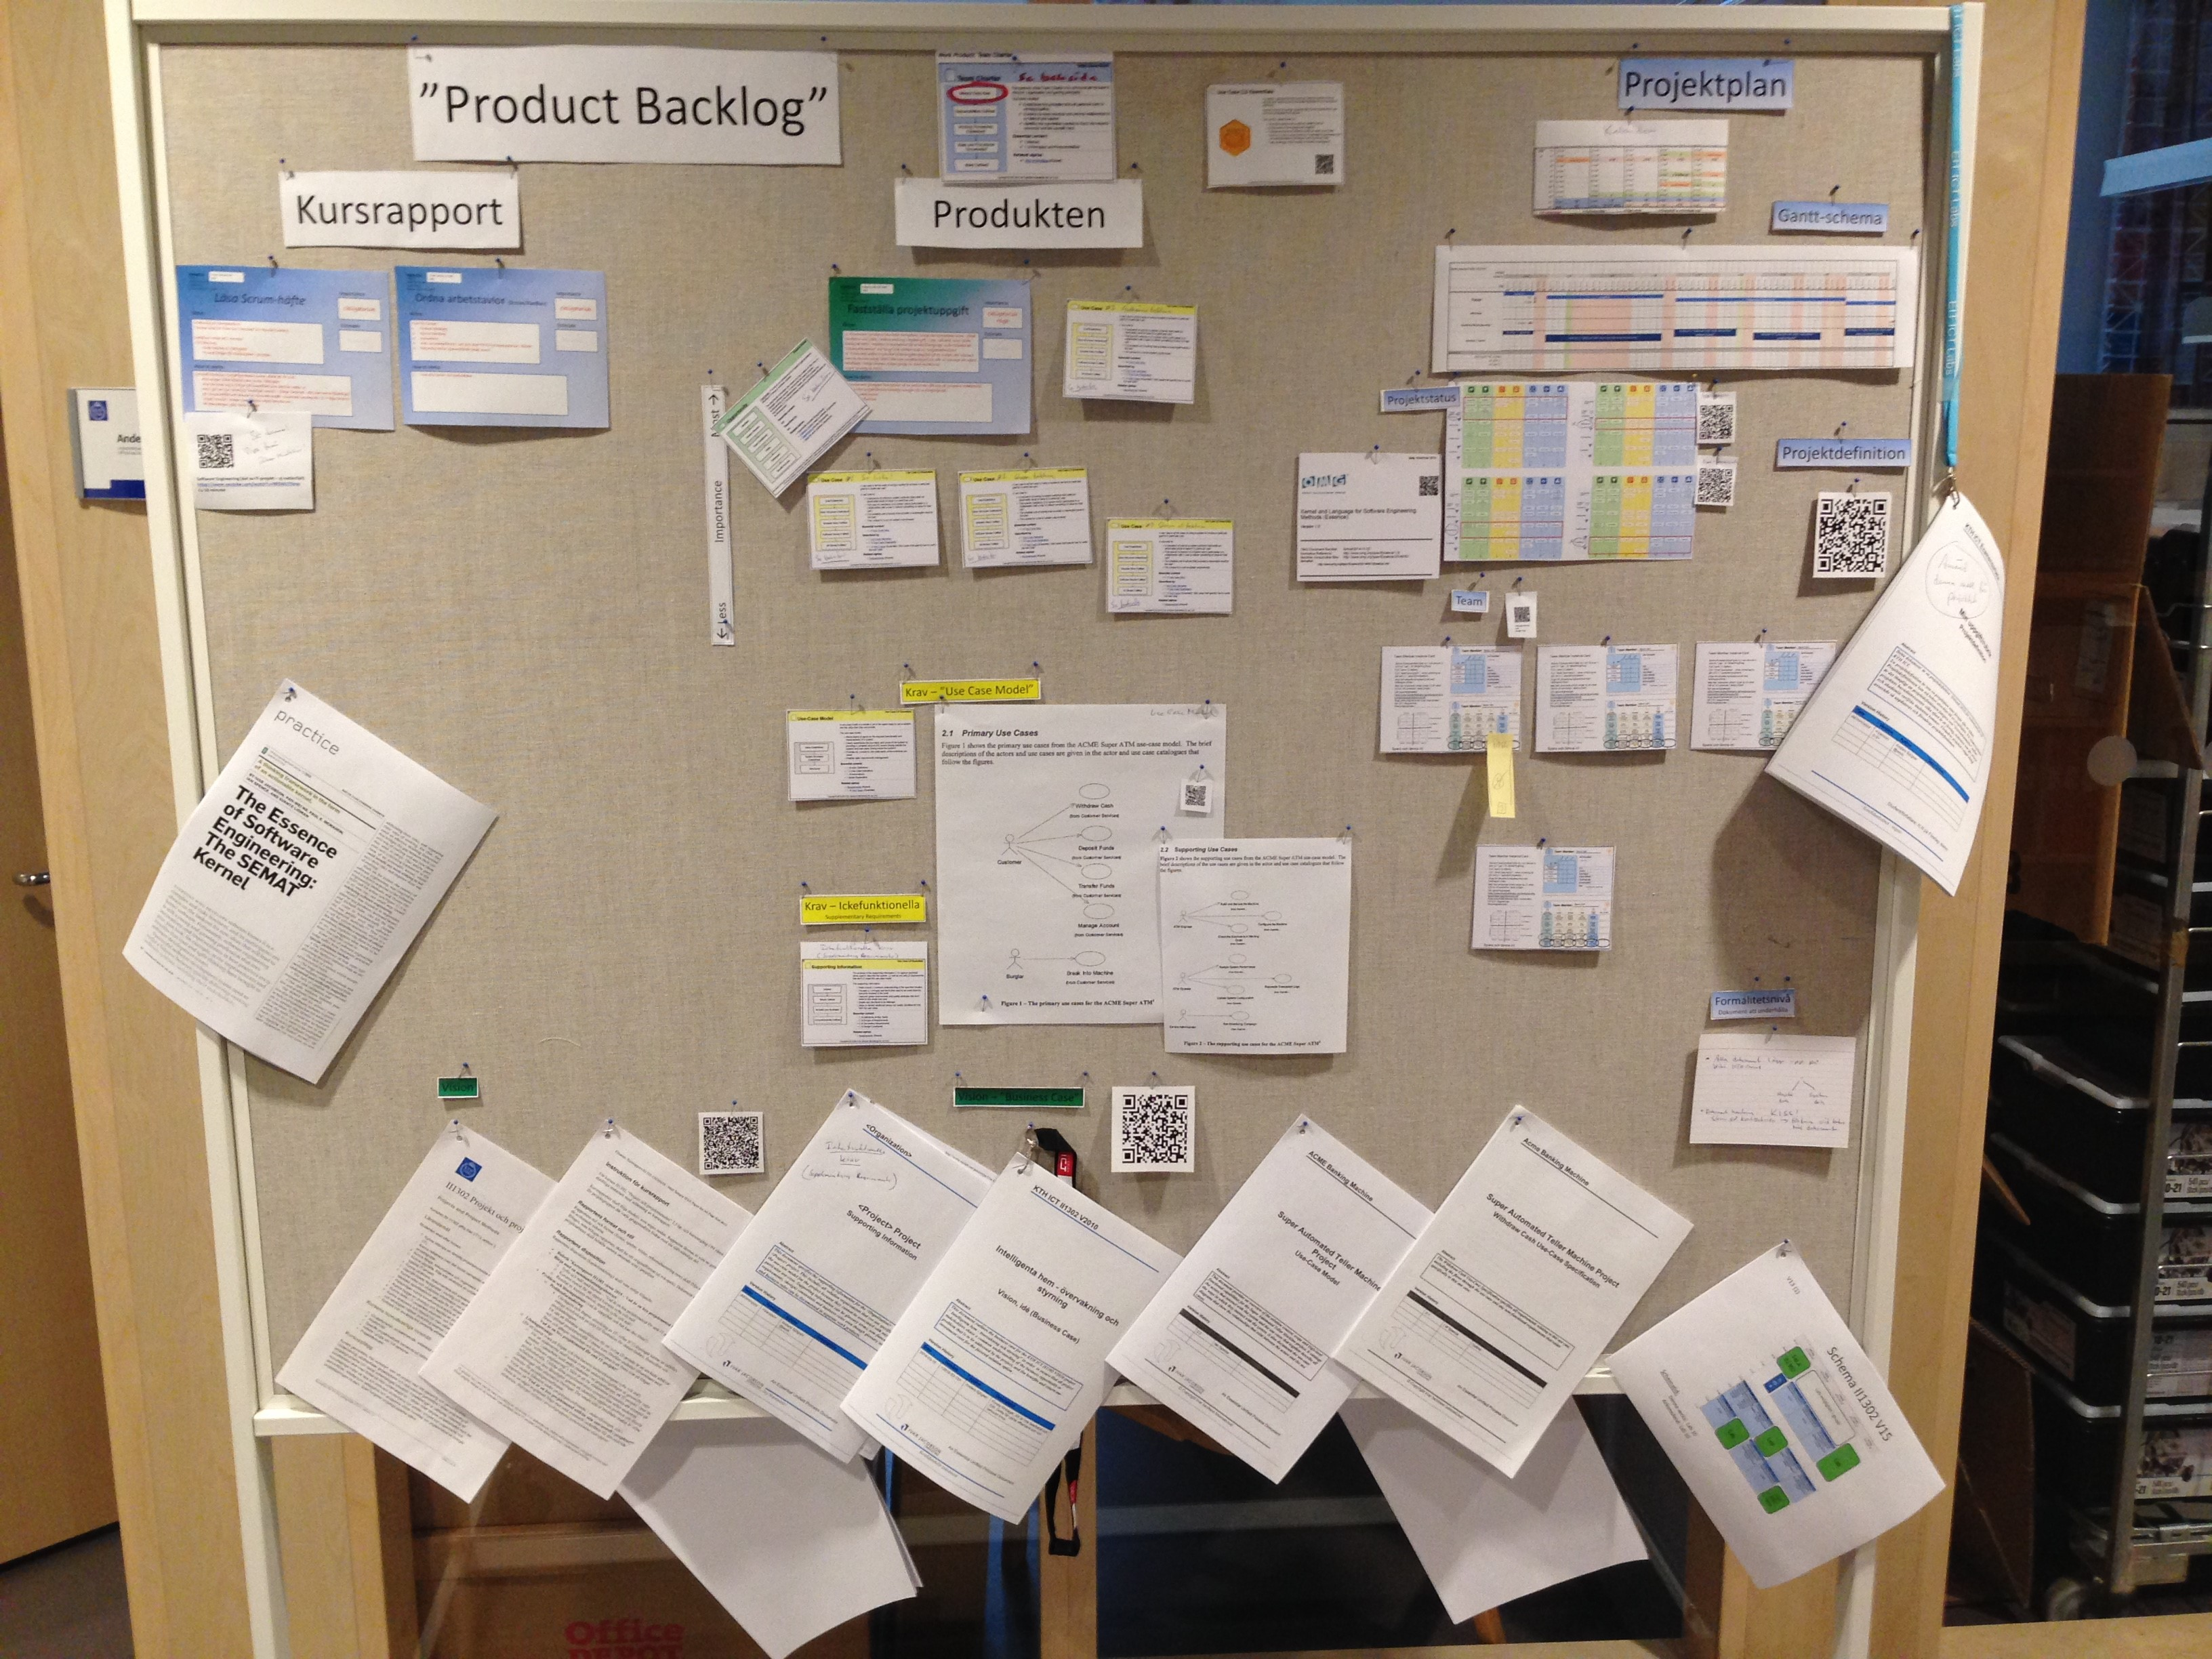
\includegraphics[max height=250px, max width=250px]{images/arbetstavla.jpg}}
        \caption{Arbetstavla "nåldyna"}
        \label{fig}
    \end{figure}
    
    \begin{figure}[htbp]
        \centerline{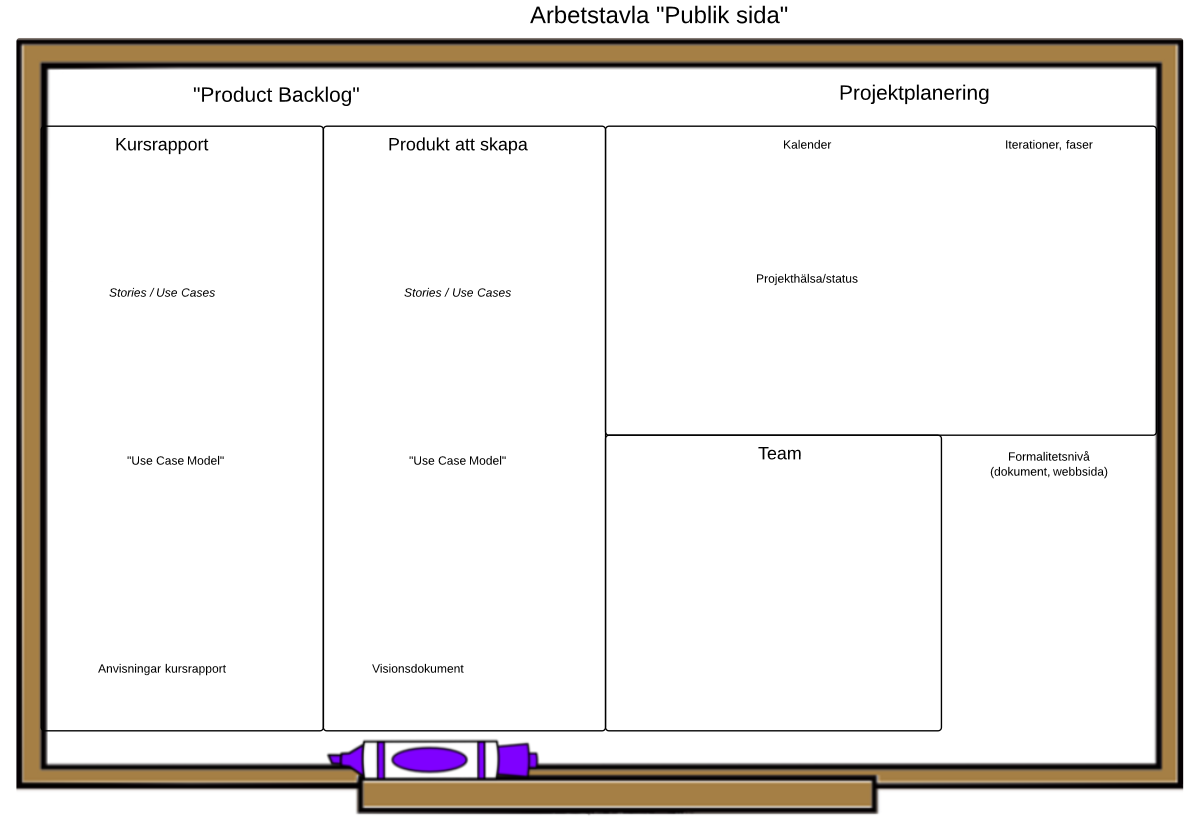
\includegraphics[max height=250px, max width=250px]{images/lucidtavla.png}}
        \caption{Arbetstavla "whiteboard" "Publik sida"}
        \label{fig}
    \end{figure}

    \begin{figure}[htbp]
        \centerline{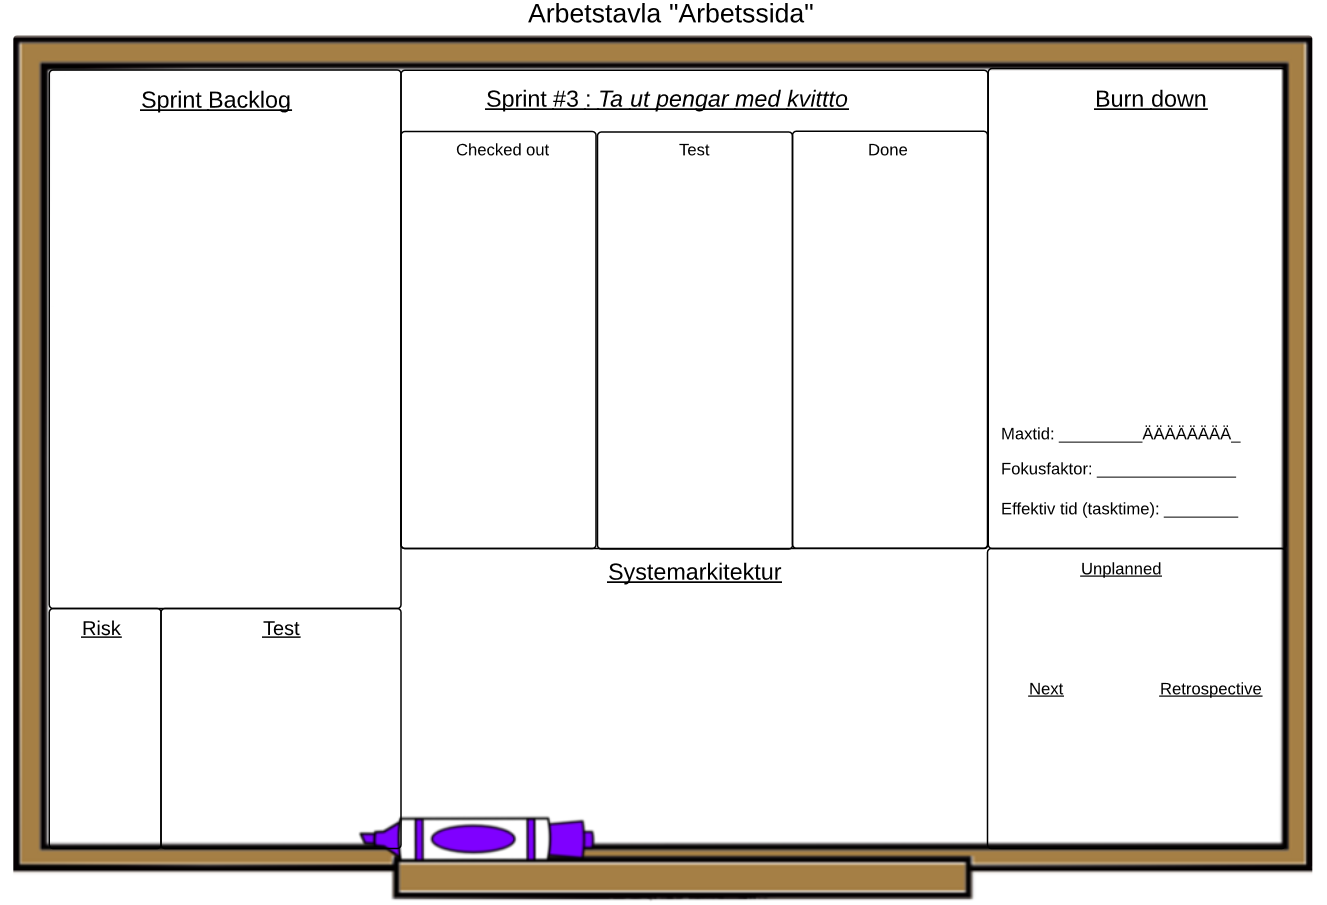
\includegraphics[max height=250px, max width=250px]{images/lucidbaksida.png}}
        \caption{Arbetstavla "whiteboard" "Arbetssida"}
        \label{fig}
    \end{figure}
    \item \textit{Scruminspirerade projektaktiviteter}
    Bilden nedan visar projektmodellens aktiviteter och ordning.

    \begin{figure}[htbp]
        \centerline{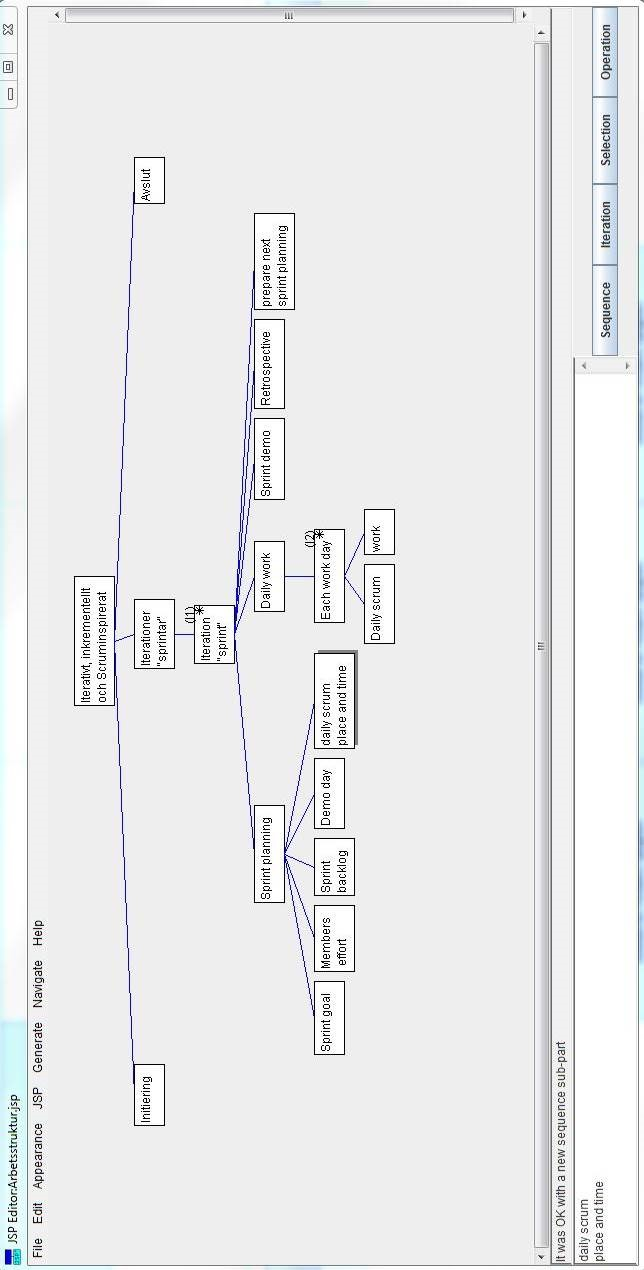
\includegraphics[max height=250px, max width=250px]{images/scrum.jpg}}
        \caption{Den här har ingen beskrivning i mallen.}
        \label{fig}
    \end{figure}
\end{enumerate}

\section{Undersökningsmetoder}
Detta kapitel beskriver vilka metoder som använts i undersökningen. Metoderna är
valda och specifierade så att de skall kunna ge svar på ett antal följdfrågor som
identifierats i denna undersökning. Först anges frågorna och sedan följer
metodbeskrivning.

\subsection{Frågor att besvara i undersökningen}
Frågorna kategoriseras i följande kategorier... (eventuellt)
\begin{enumerate}
    \item Hur skall man bedöma/redovisa om en delprojektmetod eller praktik är bra?
    \item Hur kan man kategorisera, välja och namnge projektmetoder (projektpraktiker)
    och (verklighetsbeskrivning) så att diskussionen om dito blir begreppsmässigt
    konsistent för ingenjörer inom IT-området (s.k. ontologi?).
    \item Vilka ansvarsroller skall användas som ansats i projektet?
    \item Vad består ett projekt av och vilka metoder/praxis skall användas, undersökas
    och bedömas? Vilken ansats skall göras?
    \item (Vad och hur skall eller behöver jag som student redovisa i rapporten för att
    bli godkänd på kursen? Denna fråga tas bort i den slutliga rapporten)
\end{enumerate}

\subsection{Metodbeskrivning (undersökningsmetod)}
Den centrala metoden i undersökningen är att avgöra om olika valda projekt-praktiker 
och arbetssätt är ”bra” och om de bidrar till att göra hela projektprocessen bra. 
Åstadkommer/skapar projektet rätt saker och konstrueras lösningar på bästa sätt? 
Metoden för att samla data i denna fråga blir induktiv då erfarenheten i gruppen är 
ytterst liten. Arbetssättet blir att efterhand som projektet fortskrider så förs 
bedömningsområden som anses vitala och bedömningskriterier in i en tabell kontinuerligt. 
Tabellen, se kapitel ”Resultat”, dess innehåll och dess utformning förbättras också hela 
tiden.\\

\textbf{Metod 1: Undersökningsmetod}, se figur nrX. De gula fälten är aktiviteter som 
kopplar till själva undersökningen. Metoden följer principer för vetenskaplighet 
enligt Andersson och Ekholm.
 
\begin{figure}[htbp]
    \centerline{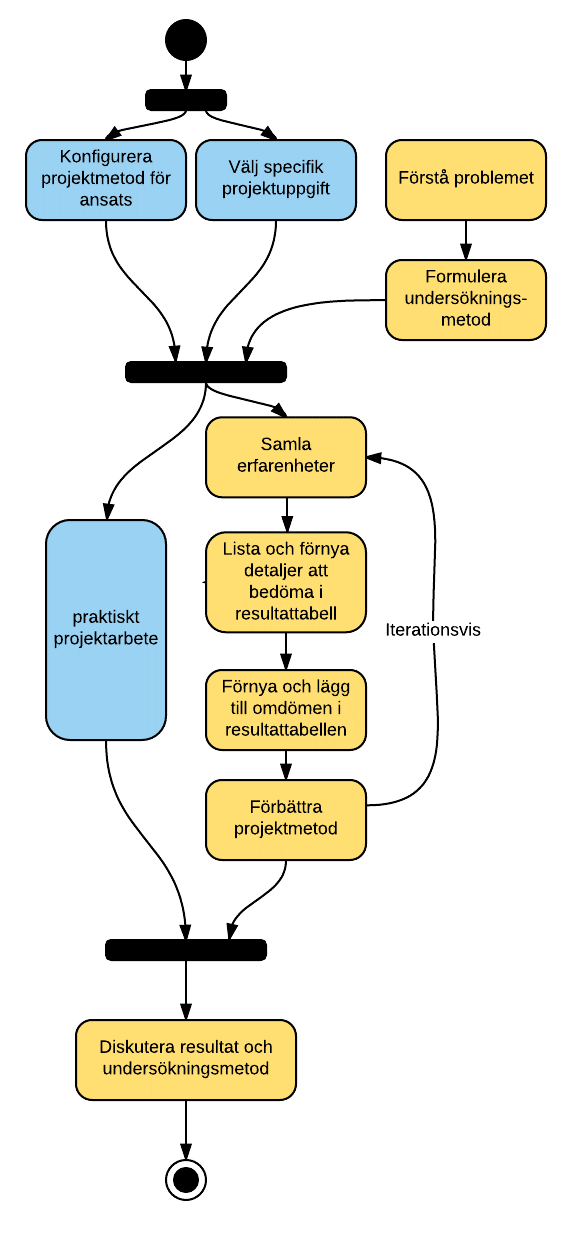
\includegraphics[max height=250px, max width=250px]{images/undersokningsmetod.png}}
    \caption{Undersökningsmetod för "Vad är bra projektmetod för små IT-projekt"}
    \label{fig}
\end{figure}

\textbf{Metod 2: Begrepp}
Begrepp som används följer om möjligt OMGs standard 
\textit{Essence - Kernel and Language for Software Engineering Methods Version 1.0}.

Följande bilder listar illustrativt centrala begrepp. I denna artikel kommer de engelska
begreppen att fritt översättas till svenska då risken för missförstånd anses liten.

\begin{figure}[htbp]
    \centerline{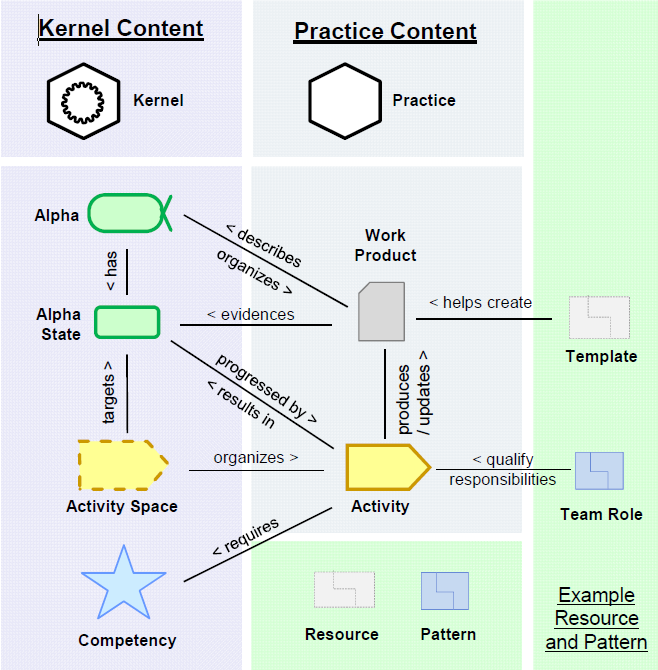
\includegraphics[max height=250px, max width=250px]{images/begrepp.png}}
    \caption{Begrepp}
    \label{fig}
\end{figure}

\begin{figure}[htbp]
    \centerline{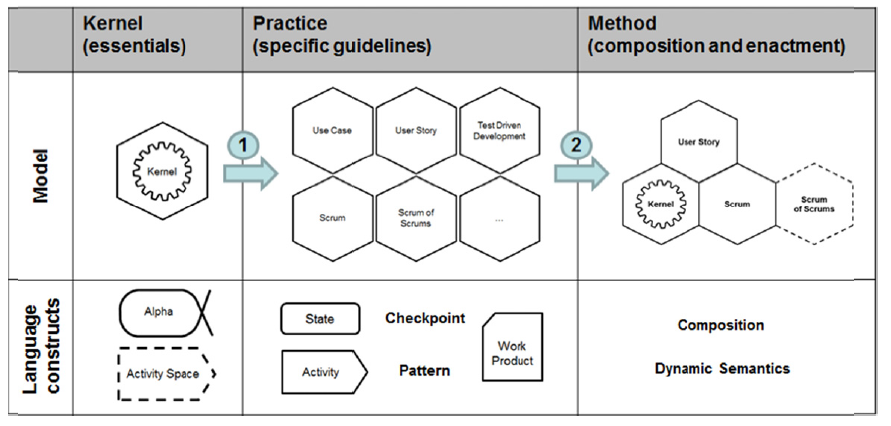
\includegraphics[max height=250px, max width=250px]{images/practicemethod.png}}
    \caption{Practice and Method}
    \label{fig}
\end{figure}

\section{Genomförande}
I följande kapitel redovisas viktiga beslut, förändringar och anpassningar som gjorts 
i projektmetod, projektpraktiker, värderingar, beslut mm som gjorts under studiens genomförande.
(Här kan det vara lämpligt med en indelning i olika ansvarsområden inom projektet?)

\subsection{Projektledning (Stina)}
Genomförandet av iterationer följer helt och hållet mallen för s k ”sprint” i Scrum [ref] 
och beskrivs enklast med följande aktivitetsdiagram, se  bild
\begin{figure}[htbp]
    \centerline{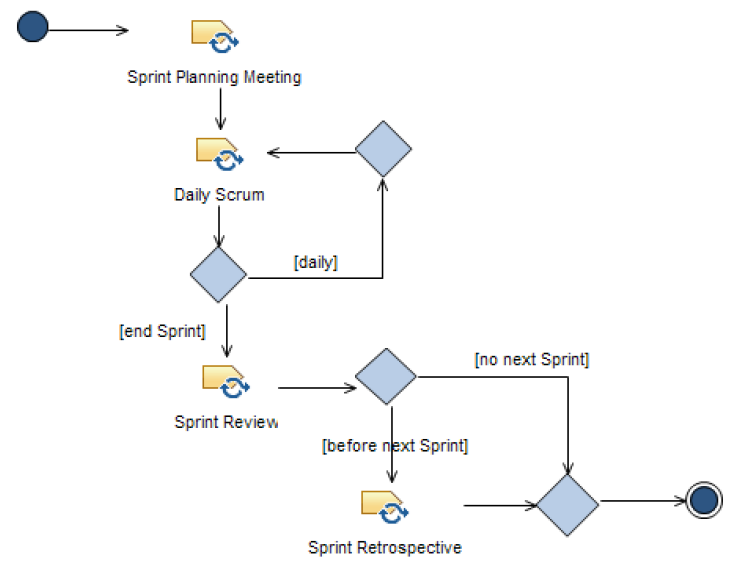
\includegraphics[max height=250px, max width=250px]{images/sprint.png}}
    \caption{Iteration/Sprint}
    \label{fig}
\end{figure}

\subsection{Kundrepresentant (Kurs)}
Lite innehåll.

\section{Resultat}
Tabellen nedan listar bedömda ”områden” och subjektiv värdering gentemot deras bidrag 
till Åstadkommer/skapar projektet rätt saker (validitet) och konstrueras lösningar på 
bästa sätt (reliabilitet)? Alternativa arbetssätt och del-projektmetoder anges också.

Fullständiga tabeller finns i bilagor. Där finns också den evidens som ligger till 
grund för listade omdömen. Positiva omdömen anges med grönt, negativa med rött och 
neutrala omdömen med gult. 

% Here you can define your own colors to use in the table. 
\definecolor{green}{RGB}{146,208,80}
\definecolor{pink}{RGB}{251,212,180}
\definecolor{yellow}{RGB}{255,255,0}
\definecolor{grey}{RGB}{217,217,217}
\begin{table}[htbp]
\caption{Bedömningar}
\begin{center}
\begin{tabular}{|l|l|l|l|}
\hline
\textbf{Ansvars-}   & \textbf{Arbetssätt/metod}     & \textbf{Omdöme}       & \textbf{Alternativ} \\
\textbf{område}     & \textbf{praktik/mönster}      & Fördelar och          & \\
                    &                               & nackdelar             &  \\
\hline
Projekt-            &                               &                       & \\
övergripande        &                               &                       & \\
\hline
Projekt-            &                               &                       & \\
ledning             & Iterativt                     & \cellcolor{green}     & \\
\hline
Analytiker          & Arkitektur                    &                       & \\
\hline
                    &                               & \cellcolor{pink}      & \\
\hline
                    &                               & \cellcolor{yellow}    & \\
\hline
                    &                               &                       & \\
\hline
\end{tabular}
\label{tab1}
\end{center}
\end{table}

\begin{table}[htbp]
\caption{"Keep - Problems - Try"\\\textit{Roll - student}}
\begin{center}
\begin{tabular}{|c|c|c|c|}
\hline
\multicolumn{4}{|c|}{\cellcolor{grey}\textbf{"Keep"}}\\
\hline \rowcolor{grey}
\textbf{"Keep"}                         & \textbf{Motivation}      & \textbf{Förbättringar} & \textbf{Referenser} \\
\hline
                                        &                          &                     & \\
                                        &                          &                     & \\
\hline
                                        &                          &                     & \\
                                        &                          &                     & \\
\hline
                                        &                          &                     & \\
\hline
                                        &                          &                     & \\
\hline
                                        &                          &                     & \\
\hline
                                        &                          &                     & \\
\hline

% This is a separator, since the tables in the .doc-template are labeled as the same table.
\multicolumn{4}{c}{}\\

\hline
\multicolumn{4}{|c|}{\cellcolor{grey}\textbf{"Problems - Try"}}\\
\hline \rowcolor{grey}
\textbf{"Problem"}                      & \textbf{"Try what?}      & \textbf{Motivering} & \textbf{Referenser} \\
\hline
                                        &                          &                     & \\
                                        &                          &                     & \\
\hline
                                        &                          &                     & \\
                                        &                          &                     & \\
\hline
                                        &                          &                     & \\
\hline
                                        &                          &                     & \\
\hline
                                        &                          &                     & \\
\hline
                                        &                          &                     & \\
\hline

% This is a separator, since the tables in the .doc-template are labeled as the same table.
\multicolumn{4}{c}{}\\

\hline
\multicolumn{4}{|c|}{\cellcolor{grey}\textbf{"Problems - Skip"}}\\
\hline \rowcolor{grey}
\textbf{"Problem"}                      & \textbf{"Skip or}        & \textbf{Motivering} & \textbf{Referenser} \\
\rowcolor{grey}                         & \textbf{replace, why?"}  &                     &  \\
\hline
                                        &                          &                     & \\
                                        &                          &                     & \\
\hline
                                        &                          &                     & \\
                                        &                          &                     & \\
\hline
                                        &                          &                     & \\
\hline
                                        &                          &                     & \\
\hline
                                        &                          &                     & \\
\hline
                                        &                          &                     & \\
\hline
\end{tabular}
\label{tab1}
\end{center}
\end{table}

\section{Analys/Förbättringsförslag}
Finns det förslag eller räcker resultaten ovan?

\section{Diskussion}
Allmän diskussion. Vad säger resultatet om "Vad är en bra projektmetod för små IT-projekt"?

\subsection{Metoddiskussion}
Validitet
Reliabilitet

\subsection{Resultatdiskussion}
Validitet
Reliabilitet

\subsection{Bidrag till vetenskaplighet, ingenjörserfarenhet (studenterfarenhet?)}
Framtida förbättringar\dots

% A section marked with a * will not be numbered.
\section*{Slutord}
Eventuella slutord.

Berätta något om produkten ni konstruerade, ange en länk till projektets Github\cite{Eklund:2}, videopresentation?
Länka till Github, rapprt mm från ditt LinkedIn-konto som exempel på arbetsprover?\cite{DUMMY:1}

\vspace{12pt}

% You can switch citation style. ieeetran could be useful, as it is a bit more pleasing to the eyes.
\bibliographystyle{apalike}
\bibliography{references}

\end{document}
